% This is the Duke University Statistical Science LaTeX thesis template.
% It has been adapted from the Reed College LaTeX thesis template. The
% adaptation was done by Mine Cetinkaya-Rundel (MCR). Some of the comments
% that are specific to Reed College have been removed.
%
% Most of the work on the original Reed College document class and template
% was done by Sam Noble (SN). Later comments etc. by Ben Salzberg (BTS).
% Additional restructuring and APA support by Jess Youngberg (JY).
%
% See https://www.reed.edu/cis/help/latex/ for help. There are a
% great bunch of help pages there, with notes on
% getting started, bibtex, etc. Go there and read it if you're not
% already familiar with LaTeX.
%
% Any line that starts with a percent symbol is a comment.
% They won't show up in the document, and are useful for notes
% to yourself and explaining commands.
% Commenting also removes a line from the document;
% very handy for troubleshooting problems. -BTS

%%
%% Preamble
%%
% \documentclass{<something>} must begin each LaTeX document
\documentclass[12pt,twoside]{dukestatscithesis}
% Packages are extensions to the basic LaTeX functions. Whatever you
% want to typeset, there is probably a package out there for it.
% Chemistry (chemtex), screenplays, you name it.
% Check out CTAN to see: http://www.ctan.org/
%%
\usepackage{graphicx,latexsym}
\usepackage{amsmath}
\usepackage{amssymb,amsthm}
\usepackage{longtable,booktabs,setspace}
\usepackage{chemarr} %% Useful for one reaction arrow, useless if you're not a chem major
\usepackage[hyphens]{url}
% Added by CII
\usepackage{hyperref}
\usepackage{lmodern}
\usepackage{float}
\floatplacement{figure}{H}
% End of CII addition
\usepackage{rotating}

% Next line commented out by CII
%%% \usepackage{natbib}
% Comment out the natbib line above and uncomment the following two lines to use the new
% biblatex-chicago style, for Chicago A. Also make some changes at the end where the
% bibliography is included.
%\usepackage{biblatex-chicago}
%\bibliography{thesis}


% Added by CII (Thanks, Hadley!)
% Use ref for internal links
\renewcommand{\hyperref}[2][???]{\autoref{#1}}
\def\chapterautorefname{Chapter}
\def\sectionautorefname{Section}
\def\subsectionautorefname{Subsection}
% End of CII addition

% Added by CII
\usepackage{caption}
\captionsetup{width=5in}
% End of CII addition

% \usepackage{times} % other fonts are available like times, bookman, charter, palatino


% To pass between YAML and LaTeX the dollar signs are added by CII
\title{Matrix Completion Techniques For Anomaly Detection in Network Attacks}
\author{James C. Wu}
% The month and year that you submit your FINAL draft TO THE LIBRARY (May or December)
\date{May 2018}
\advisor{Peter D. Hoff}
\institution{Duke University}
\degree{Bachelor of Science in Statistical Science}
\committeememberone{Jerry P. Reiter}
\committeemembertwo{Galen Reeves}
\dus{Mine Cetinkaya-Rundel}
%If you have two advisors for some reason, you can use the following
% Uncommented out by CII
% End of CII addition

%%% Remember to use the correct department!
\department{Department of Statistical Science}

% Added by CII
%%% Copied from knitr
%% maxwidth is the original width if it's less than linewidth
%% otherwise use linewidth (to make sure the graphics do not exceed the margin)
\makeatletter
\def\maxwidth{ %
  \ifdim\Gin@nat@width>\linewidth
    \linewidth
  \else
    \Gin@nat@width
  \fi
}
\makeatother

\renewcommand{\contentsname}{Table of Contents}
% End of CII addition

\setlength{\parskip}{0pt}

% Added by CII
  %\setlength{\parskip}{\baselineskip}
  \usepackage[parfill]{parskip}

\providecommand{\tightlist}{%
  \setlength{\itemsep}{0pt}\setlength{\parskip}{0pt}}

\Acknowledgements{
I thank my advisor, Professor Peter Hoff, and the Director of
Undergraduate Studies, Professor Mine Cetinkaya-Rundel, for their
guidance in this project. I also thank Duke University's Statistics
Department for supervising this project and the Office of Information
Technology for providing the dataset. Most of all I thank my parents for
their continued unwavering support in all my endeavors.
}

\Dedication{

}

\Preface{

}

\Abstract{
The goal of this project is to identify novel methods for detecting
anomalies in network IP data. The space is represented as a
3-dimensional tensor of the continuous features (source bytes,
destination bytes, source packets, destination packets) divided by their
respective source port and destination port combinations. This project
implements and assesses the validity of principal component analysis and
matrix completion via singular value decomposition (more methods
pending) in determining anomalous entries in the tensor.
}

% End of CII addition
%%
%% End Preamble
%%
%

\usepackage{amsthm}
\newtheorem{theorem}{Theorem}[chapter]
\newtheorem{lemma}{Lemma}[chapter]
\theoremstyle{definition}
\newtheorem{definition}{Definition}[chapter]
\newtheorem{corollary}{Corollary}[chapter]
\newtheorem{proposition}{Proposition}[chapter]
\theoremstyle{definition}
\newtheorem{example}{Example}[chapter]
\theoremstyle{definition}
\newtheorem{exercise}{Exercise}[chapter]
\theoremstyle{remark}
\newtheorem*{remark}{Remark}
\newtheorem*{solution}{Solution}
\begin{document}

% Everything below added by CII
  \maketitle

\frontmatter % this stuff will be roman-numbered
\pagestyle{empty} % this removes page numbers from the frontmatter
  \begin{acknowledgements}
    I thank my advisor, Professor Peter Hoff, and the Director of
    Undergraduate Studies, Professor Mine Cetinkaya-Rundel, for their
    guidance in this project. I also thank Duke University's Statistics
    Department for supervising this project and the Office of Information
    Technology for providing the dataset. Most of all I thank my parents for
    their continued unwavering support in all my endeavors.
  \end{acknowledgements}

  \hypersetup{linkcolor=black}
  \setcounter{tocdepth}{2}
  \tableofcontents


  \begin{abstract}
    The goal of this project is to identify novel methods for detecting
    anomalies in network IP data. The space is represented as a
    3-dimensional tensor of the continuous features (source bytes,
    destination bytes, source packets, destination packets) divided by their
    respective source port and destination port combinations. This project
    implements and assesses the validity of principal component analysis and
    matrix completion via singular value decomposition (more methods
    pending) in determining anomalous entries in the tensor.
  \end{abstract}

\mainmatter % here the regular arabic numbering starts
\pagestyle{fancyplain} % turns page numbering back on

The goal of this project is to identify novel methods for detecting
anomalies in network IP data. The space is represented as a
3-dimensional tensor of the continuous features (source bytes,
destination bytes, source packets, destination packets) divided by their
respective source port and destination port combinations. This project
implements and assesses the validity of principal component analysis and
matrix completion via singular value decomposition (more methods
pending) in determining anomalous entries in the tensor.

\chapter{Introduction}\label{introduction}

\section{Anomaly Detection}\label{anomaly-detection}

Anomaly detection is used to identify unusual patterns or observations
that do not conform to expected behavior in a dataset. Anomalies can be
broadly categorized into three categories:

Point anomalies: A single instance of data is anomalous if it's too far
off from the rest. For example detecting credit card fraud based on a
single spending spree that represents the credit card being stolen and
used.

Contextual anomalies: The abnormality is context specific. This type of
anomaly is common in time-series data. For instance, high spending on
food and gifts every day during the holiday season is normal, but may be
considered unusual otherwise.

Collective anomalies: A set of data observations that when collectively
assessed helps in detecting anomalies. For instance, repeated pings from
a certain IP address to a port connection on a hosted network may be
classified as a port scanner, which often preludes a network attack.

\section{Network Attacks}\label{network-attacks}

Network security is becoming increasingly relevant as the flow of data,
bandwith of transactions, and user dependency on hosted networks
increase. As entire networks grow in nodes and complexity, attackers
gain easier entry points of access to the network. The most benign of
attackers attempt to shutdown networks (e.g.~causing a website to
shutdown with repeated pings to its server), while more malicious
attempts involve hijacking the server to publish the attacker's own
content or stealing unsecured data from the server, thus compromising
the privacy of the network's users.

Attackers follow a specific three step strategy when gathering
intelligence on a network, the most important component of which is
scanning. Network scanning is a procedure for identifying active hosts
on a network, the attacker uses it to find information about the
specific IP addresses that can be accessed over the Internet, their
target's operating systems, system architecture, and the services
running on each node/computer in the network. Scanning procedures, such
as ping sweeps and port scans, return information about which IP
addresses map to live hosts that are active on the Internet and what
services they offer. Another scanning method, inverse mapping, returns
information about what IP addresses do not map to live hosts; this
enables an attacker to make assumptions about viable addresses.

All three of these scanning methods leave digital signatures in the
networks they evaluate because they apply specific pings that are then
stored in the network logs. Most scanners use a specific combination of
bytes, packets, flags (in TCP protocol), and ports in a sequence of
pings to a network. Identifying a scanner's often many IP addresses from
the set of pings available in the network's logs is thus an anomaly
detection problem. In particular, because the data is unlabeled, meaning
it is unclear which observations are actually scanners and which are
just standard user behavior, unsupervised approaches are necessary for
tackling the problem.

This particular dataset is from Duke University's Office of Information
Technology (OIT), and it covers all observations in their network
traffic during a five minute period in February 2017.

\subsection{Status Quo Solution}\label{status-quo-solution}

OIT's current solution for detecting scanners relies on specific domain
knowledge gathered from diagnostics programs and data analysis completed
on previous data. They prevent scanners by blocking IP addresses that
fit certain rules they have constructed to run on every network
transaction as it occurs. The specific checks in these rules are private
for security reasons, but they belong to the nature of evaluating the
size of transactions, repeated connections between particular ports,
many pings from the same address, and combinations of these particular
behaviors.

While this solution presents a methodical way for banning IP addresses
and its method of rule checking is essentially removing what OIT
considers outliers for network transactions-any observation that does
not fit within the constraints specified by the rules is classified as
an outleir and its source IP is blocked-it is inflexible, prone to
detecting false negatives, and fails to detect observations that may be
within the parameter constraints of the rules but are anomalous with
respect to other parameters or parameter constraints.

\section{Network Dataset}\label{network-dataset}

\subsection{Features}\label{features}

The networks dataset contains 13 features, 8 categorical and 5
continuous, and the observations are unlabeled (not specified whether
they are considered a scanner). The 13 features are:

\textbf{Continuous:}
\begin{itemize}
\tightlist
\item
  StartTime (Start Time): the time when the observation is logged
\item
  SrcBytes (Source Bytes): the total number of bytes sent in the
  observation
\item
  SrcPkts (Source Packets): the number of packets sent in the
  observation
\item
  DstBytes (Destination Bytes): the total number of bytes received in
  the observation
\item
  DstPkts (Destination Packets): the number of packets received in the
  observation Note, the destination packets and bytes features do not
  have the same values as their source counterparts because the
  connections are compressed and decompressed into different forms and
  byte sizes when sent. For instance, it is possible for the number of
  destination packets to be larger than source packets. It is also
  possible for information to be lost during the connection.
\end{itemize}
\textbf{Categorical:}
\begin{itemize}
\tightlist
\item
  Flgs (connection flag): flow state flags seen in transaction between
  the two addresses
\item
  Proto (network protocol): specifies the rules used for information
  exchange via network addresses. Transmission Control Protocol (TCP)
  uses a set of rules to exchange messages with other Internet points at
  the information packet level, and Internet Protocol (IP) uses a set of
  rules to send and receive messages at the Internet address level.
\item
  SrcAddr (Source Address): the IP address of the connection's source
\item
  DstAddr (Destination Address): the IP address of the connection's
  destination
\item
  Sport (Source Port): the network port number of the connection's
  source. A port numbers identifies the specific process to which a
  network message is forwarded when it arrives at a server.
\item
  Dport (Destination Port): the network port number of the connection's
  destination
\item
  Dir (direction): the direction of the connection
\item
  State (connection state): a categorical assessment of the current
  phase in the transaction when the timestamp is recorded
\end{itemize}
Note, the addresses have been anonymized for security reasons.

\subsection{Argus}\label{argus}

Argus is the open source network security tool applied to network
transactions that collects the data for the features. The Argus wiki and
the OIT manual provides key insights into the structure and nature of
the data. Specifically, the sessions are clustered together by address,
so the pytes and packets values are accumulative over a set duration and
each session has its own start time but does not have a tracked end
time. There exist 2-4 million connections on average every 5 minutes.
Furthermore the protocol in this dataset is always gathered from TCP
protocol and the direction will always be to the right (i.e.~Source to
Destination). This information supports dropping proto, StartTime, and
Direction from the dataset for future analysis because they do not
present any information regarding whether an observation can be
considered an anomaly. Furthermore, the State feature may not be
reliable because Argus occasionally resets the state data statistics
during monitoring.

\chapter{Modeling Port Relationships}\label{modeling-port-relationships}

\section{Motivation}\label{motivation}

Preliminary data analysis signaled that there may exist trends between
different port combinations. For instance, a particular source and
destination port may frequently contain large byte transactions in their
connections. Devising a systematic way to identify these combinations
may present outliers that can be further investigated for scanner
behavior.

This approach to the anomaly detection problem reduces the dataset to
the values of the four continuous features, SrcBytes, SrcPkts, DstBytes,
DstPkts, observed across different source port and destination port
combinations. The data can be represented as a 3-dimensional tensor
\(Y \in \mathbb{R_{m \times n \times 4}}\) where \(m\) represents the
number of source ports, \(n\) represents the number of destination
ports, and \(4\) accounts for the four continuous features in the
dataset. Each cell, \(y_{ijk}\), contains the mean of all the
observations observed for source port, \(i\), and destination port
\(j\). In the cases where the combination of \(i\) and \(j\) is not
observed in the dataset, \(y_{ijk}\) is missing.

The goal of this paper is to devise an optimal strategy for imputing the
missing cells in \(Y\) to create the completed tensor
\(Y' \in \mathbb{R_{m \times n \times 4}}\). As new observations are
observed for combinations of ports \(i\) and \(j\), the \(y'_{ijk}\)
values can be interpreted as an approximation for the expected behavior
for that particular port combination. Observations with continuous
features that are a certain threshold away from \(y'_{ijk}\) may be
marked as anomalies and investigated further.

Imputing values for each of the four continuous features in the dataset
for all possible source and destination port combinations yields a
reasonable expected value in each cell of the ports matrix that can then
be compared to actual connection values when they are observed. New
observations that differ greatly from the imputed values are flagged as
anomalies and require further investigation.

\section{Tensor Properties}\label{tensor-properties}

The following properties of \(Y\) inform the imputation strategies in
following sections.

\subsection{Correlations}\label{correlations}

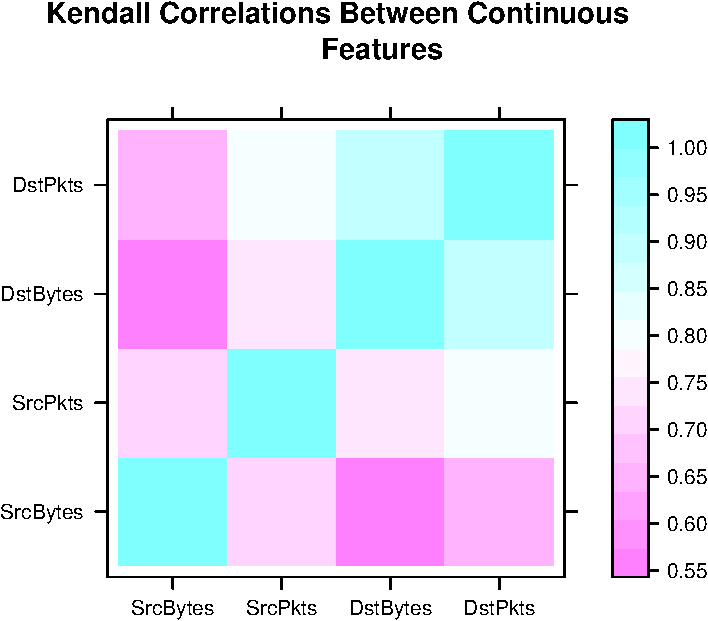
\includegraphics{thesis_files/figure-latex/unnamed-chunk-2-1.pdf}

The matrix above describes the Kendall rank correlations (commonly
referred to as Kendall's tau coefficent) between the four continuous
features in the dataset.

Intuitively, the Kendall correlation between two features will be high
when observations have a similar rank (i.e.~relative position label of
observations within the variable: 1st, 2nd, 3rd, etc.) between the two
variables, and low when observations have a dissimilar rank between the
two variables. The range of correlations is {[}-1, 1{]}. Kendall
correlation was selected as a measure because it evaluates ranks between
observations, as opposed to Pearson, which is more susceptible to
outliers in the dataset (large byte and packet observations in the
continuous feautres skewed the Pearson measures).

\subsection{Missingness}\label{missingness}

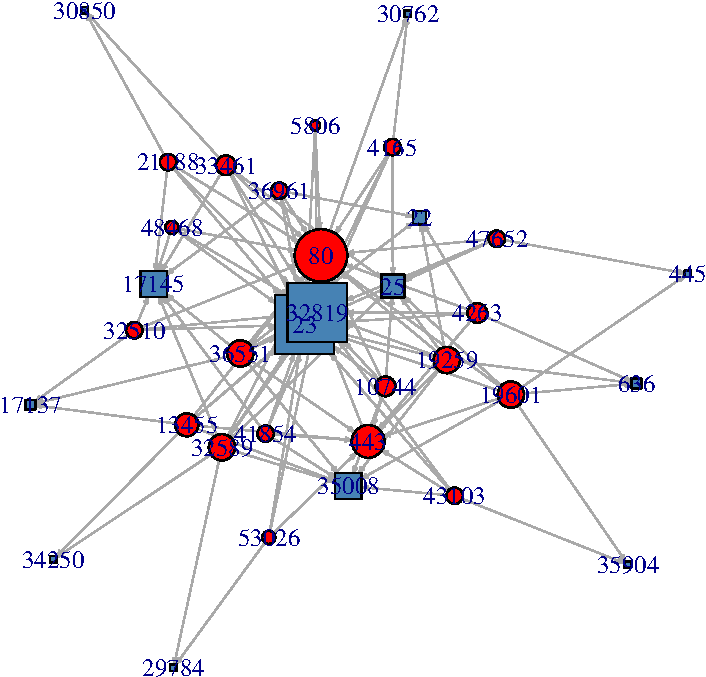
\includegraphics{thesis_files/figure-latex/unnamed-chunk-3-1.pdf}

The above matrix represents the missingness in the port combinations for
pairings of the top 20 most used source ports and destination ports. The
black cells represent missingness; of the 400 cells in the matrix, 295
(73.75\%) of cells are missing observations.

\subsection{Row and Column Properties}\label{row-and-column-properties}

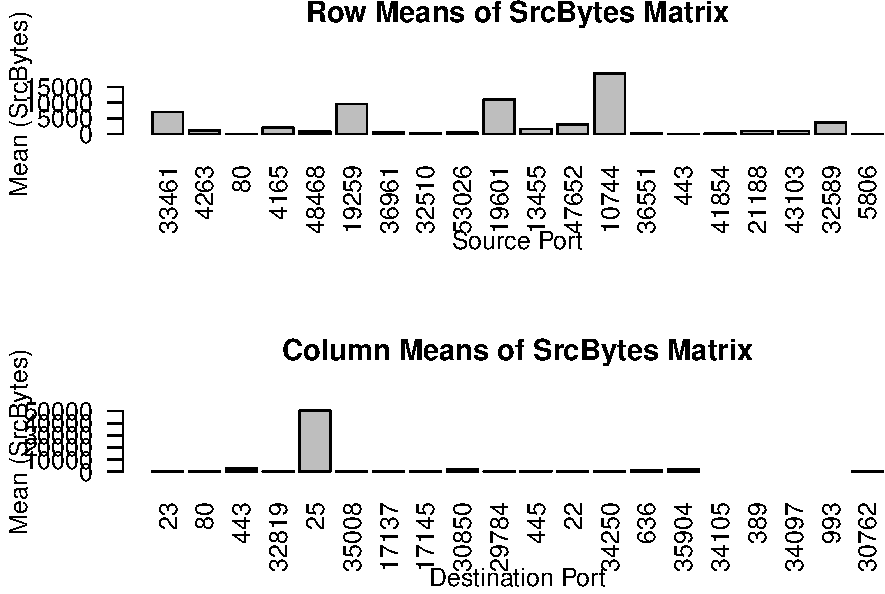
\includegraphics{thesis_files/figure-latex/unnamed-chunk-4-1.pdf}

The bar plots above represent the row and column means of the continuous
features for each slice of the tensor. These row means and column means
inform imputation techniques for the missing cells within those
respective rows and columns. COMMENT ON DISPROPORTIONATE MEANS BASED ON
MISSING VARIANCES

\subsection{Port Connections}\label{port-connections}

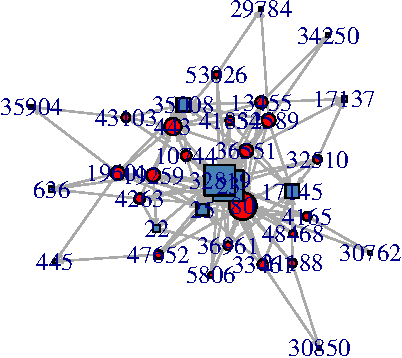
\includegraphics{thesis_files/figure-latex/unnamed-chunk-5-1.pdf}

Describe Ports network graph

\subsection{Matrix Slice Properties}\label{matrix-slice-properties}

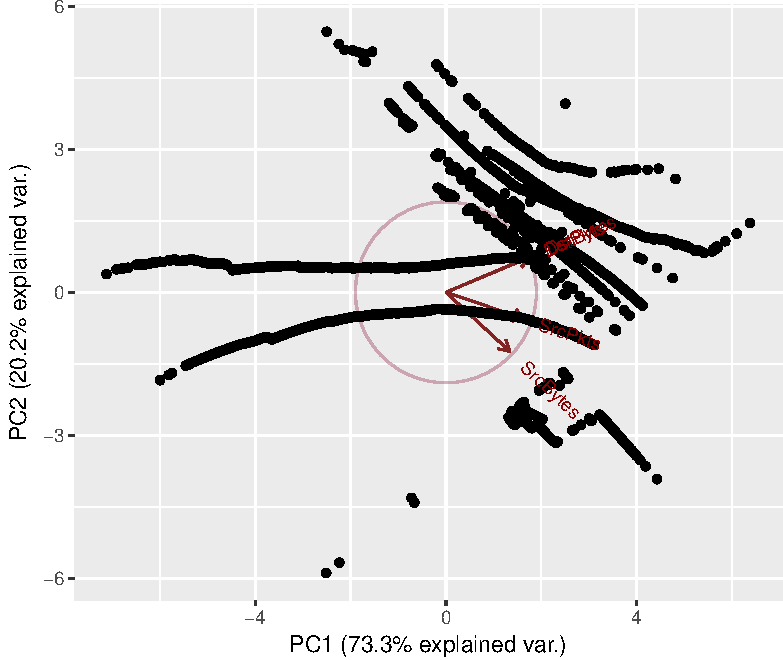
\includegraphics{thesis_files/figure-latex/unnamed-chunk-6-1.pdf}

Variance in sample size 0 to 35000

\chapter{Alternating Least Squares Applied to Two Dimensional
Matrices}\label{alternating-least-squares-applied-to-two-dimensional-matrices}

\section{Motivation}\label{motivation-1}

The preliminary tensor imputation technique slices the tensor into four
separate matrices,
\(Y^{(1)}, Y^{(2)}, Y^{(3)}, Y^{(4)} \in \mathbb{R}_{m \times n}\). Each
matrix has dimensions defined by the number of source ports by the
number of destination ports. Each cell, \(Y^{(k)}_{ij}\) contains the
mean of the observations observed for continuous feature \(k\) and
source port \(i\) destination port \(j\). Each matrix will have its
missing cells imputed with information from the rest of that matrix, and
separately from information about the other matrices. The four completed
matrices will then be recombined to create the tensor \(Y\). Similar
techniques for matrix completion were employed in the Netflix Challenge
where top competitor predicted ratings for movies by users that had not
watched the movie based on the other ratings in the matrix of users and
movies.

\section{Matrix Completion Algorithm}\label{matrix-completion-algorithm}

Each \(Y^{(k)}\) has missingness because not every source port interacts
with every destination port. \(F \in \mathbb{R}_{m \times n}\) is a
sparse matrix that represents the frequencies of combinations, i.e
\(F[32242,12312]\) represents the number of observations for the 32242
12312 port interaction. \(M \in {\rm I\!R}^{m \times n}\) represents a
boolean matrix of whether the corresponding \(Y\) values are missing.
\(Y^{(k)}[M]\) represents all of the missing values of \(Y^{(k)}\).
Moreover because each non-missing observation contains all four
continuous features, \(Y[M]\) represents all the missing values of
\(Y\).

The objective is
\[min \sum_{i,j:F_{i,j} > 0} (Y^{(k)}_{i,j} - u^{(k)}_iD^{(k)}v^{(k)T}_j)^2\]
where \(U^{(k)}D^{(k)}V^{(k)T}\) represents the singular value
decomposition of \(Y^{(k)}\). There are multiple steps to the matrix
completion process:

\subsection{ANOVA Initial Imputation}\label{anova-initial-imputation}

Impute the initial values for the missing \(y^{(k)}_{i,j}\) observations
\(1 \leq i \leq m, 1 \leq j \leq n\): In general an additive model is
applicable:
\[y^{(k)}_{i,j} = \mu^{(k)} + a^{(k)}_i + b^{(k)}_j + \epsilon^{(k)}_{i,j}\]
where \(\epsilon^{(k)} \in N(0,\sigma^2)\), \(\mu^{(k)}\) is the overall
mean of \(Y^{(k)}\), \(a^{(k)}_i\) is the row mean, and \(b^{(k)}_j\) is
column mean. An analysis of variance (ANOVA) imputation is used to fill
in the initial values, \(y^{(k)}_{i,j}\). Ignoring the missing values
for now, let \(y_{..}\) denote the empirical overall mean, \(y_{i.}\)
denote the empirical row mean, and \(y_{.j}\) denote the column mean.
\[y_{i,j} = y_{..} + (y_{i.}-y{..}) + (y_{.j}-y_{..}) = y_{i.} + y_{.j} - y{..}\]

\subsection{Repeated Imputation}\label{repeated-imputation}

The repeated imputation procedure solves
\(Y^{(s)}[M] = R_k(Y^{(s-1)})[M]\) where \(R_k\) is the best rank-k
approximation for the \(s\)-th step. For each step \((s)\) use singular
value decomposition to decompose \[Y^{(s)} =  U^{(s)}DV^{T(s)}\] where
\(D\) is a diagonal matrix of the singular values, \(U\) is the left
singular vectors of \(Y\) and \(V\) is the right singular vectors of
\(Y\).

The Eckart-Young-Mirsky (EYM) Theorem provides the best rank-k
approximation for the missing values in \(Y^{(s+1)}\). Recall \(Y[M]\)
represents all of the missing values of \(Y\). Applying the EYM theorem:
\[Y^{(s+1)}[M] = (U[,1:k]^{(s)}D[,1:k]V[,1:k]^{T(s)})[M]\] Where
\(U[,1:k]\) represents the first \(k\) columns of \(U\) and the same for
\(D\) and \(V\).

\subsection{Convergence Criterion}\label{convergence-criterion}

The EYM rank approximation imputation steps are repeated until the
relative difference between \(Y^{(s+1)}\) and \(Y^{(s)}\) falls below a
set threshold, \(T\). The relative difference threshold is expressed:
\[\frac{\|Y^{(s+1)}-Y^{(s)}\|_2}{\|Y^{(s)}\|_2} < T\] where \(\|Y\|_2\)
is the Frobenius norm. The denominator of the expression ensures the
convergence criterion is invariate to a scale change in the matrix
itself.

\subsection{Implementation}\label{implementation}

\subsection{Leave One Out Cross
Validation}\label{leave-one-out-cross-validation}

To assess the quality of the imputation, Leave-One-Out Cross Validation
(LOOCV) is used to generate a prediction error. LOOCV cycles through the
observed values, setting each to NA (missing), and then performing the
described imputation process. The prediction error is then calculated as
some function of the difference between the imputed value and the true
value. In this case, the algorithm records absolute error
\(\sum \mid \hat y_{i,j} - y_{i,j}\mid\) and root mean square error
\(\sqrt{\frac{\sum (\hat y_{i,j} - y_{i,j})^2}{n}}\) where \(n\) is the
number of observations not missing.

\section{Validation Against Simulated
Data}\label{validation-against-simulated-data}

Before applying the algorithm on the real data it is useful to validate
the algorithmic approach against simulated data where the true rank is
known.

\subsection{Simulating a Low Rank
Matrix}\label{simulating-a-low-rank-matrix}

Taking the Kronecker product of two lower dimension matrices yields a
higher dimension matrix with low rank. Explicitly, given matrix
\(A \in \mathbb{R}_{m \times r}\) and \(B \in \mathbb{R}_{r \times n}\),
\(A \otimes B = C\) where \(C \in \mathbb{R}_{m \times n}\) with rank
\(r\). Thus, when \(r < m, r < n\) the matrix \(C\) has an optimal low
rank that minimizes the root mean square error from the leave one out
cross validation procedure. To add noise to the simulated matrix, \(C\),
simply add an error matrix, \(E \in \mathbb{R}\) where
\(e_{i,j} \sim N(0,1)\).

Moreover, this procedure provides a computationally efficient way to
simulate many random low rank matrices to use as inputs for the
validation procedure. In the case of simulated matrices, there is no
missing entries, so the leave one out cross validation procedure
sequentially removes each cell in the matrix, imputes its value using
the rank being investigated, and considers the error as a function of
the difference between the true value and the imputed value.

WHAT PLOTS OR VISUALIZATIONS DO I USE FOR RESULTS? HISTOGRAM OF
PERCENTAGES FOR RANK APPROXIMATIONS? 1-4 100\%, higher ranks arent that
relevant; effects of noise

USE THIS TECHNIQUE TO SHOW DIFFERENT EFFECTS OF NOISE?

\subsection{Approximating Optimal
Rank}\label{approximating-optimal-rank}

\section{Results on Real Data}\label{results-on-real-data}

The above plot displays the root mean square errors from leave one out
cross validation across different rank inputs into the algorithm. It's
clear that rank 2 provides the best low-rank solution for the
alternating least squares imputation algorithm. Thus rank 2 is used in
the algorithm to impute the missing values in \(Y\).

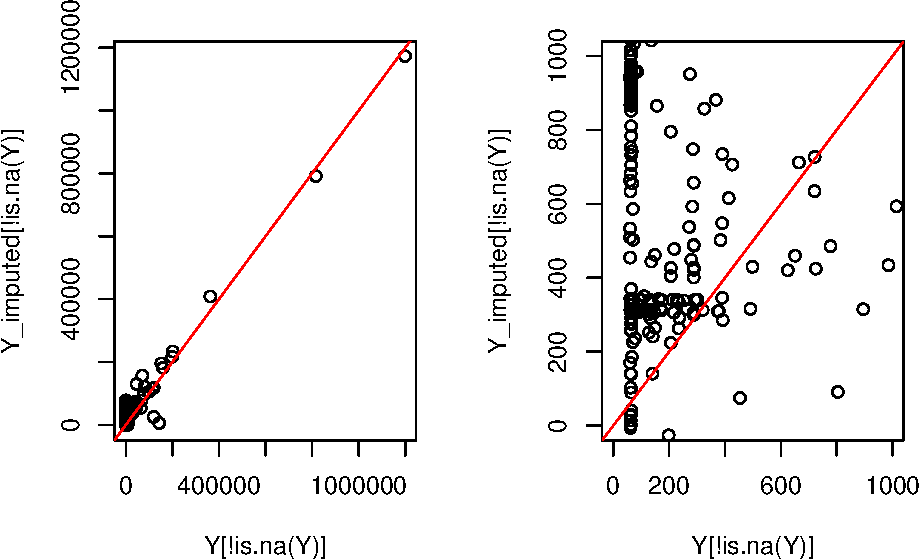
\includegraphics{thesis_files/figure-latex/unnamed-chunk-12-1.pdf}

The two plots above display the true values of the \(Y\) matrix
(i.e.~the non-missing values) versus their corresponding fitted values
using the alternating least squares algorithm with an input of rank 2.
The first plot displays all values and shows a somewhat positive linear
trend (an ideal fit of the true values would be a scatter of points
following the 45 degree angled line represented in red). However,
several outliers with large true values skew this dataset and cause the
plot to appear linear. Closer examination of the true and fitted values
smaller than 1000 (the plot on the right) reveals the relationship is
far from the linear pattern.

\subsection{Scale Transformations}\label{scale-transformations}

The poorly fitted results motivates a consideration of the scale of the
data. The present algorithm uses the sample averages of the overall
matrix as well as the row and column means when imputing each missing
cell value. This reliance upon sample means leads to susceptiblity to
outliers. Moreover exploratory data analysis reveals the dataset
contains outliers, particularly in the SrcBytes and DstBytes
measurements. Thus, a transformation of features in the model may be
appropriate for improving the fit of the algorithm.

When a natural log transformation is applied to the raw dataset before
any imputation steps are taken, the alternating least squares imputation
algorithm yields the following root mean square errors varied by rank.
Note, these errors have been reverse transformed with exponentiation to
remain on the same scale as the errors from the non-transformed dataset.

\chapter{A Bayesian Approach to Two Dimensional Matrix
Completion}\label{a-bayesian-approach-to-two-dimensional-matrix-completion}

\section{Motivation}\label{motivation-2}

The previous section's results reflected the need for an imputation
strategy that accounted for the variability in the number of
observations observed for each port combination when imputing that
particular combination's cell. The previous technique fails to take into
account the differing sample size and variance in each cell (source port
\(i\), destination port \(j\)), so the algorithm treated each
\(y_{ij}^{k}\), which represents the mean of all observations in cell
\((i,j)\) for continuous feature \(k\), as a single value with no
consideration of differing sample sizes and variances between cells. The
following section constructs a statistical model that takes frequency of
observations for each cell into account and repeatedly samples from that
statistical model to complete the matrix.

\section{Statistical Model for Port
Relationships}\label{statistical-model-for-port-relationships}

Additive Main Effects and Multiplicative Interaction Models (AMMI
models) provide a defined statistical model for each cell in the ports
matrix. In particular, the model combines the additive effects of the
initial ANOVA imputation with the multiplicative effects yielded from
singular value decomposition described in the previous section. More
importantly, the model also includes a variance term for each cell that
takes into account the differing frequency of observations in each port
combination.

The following statistical model is defined for imputing port
relationships:
\[y_{i,j} = u_i^Tv_j + \frac{\sigma_i \tau_j}{\sqrt{n_{ij}}}\epsilon_{ij}\]
where \(u_i\) represents \_\_\_\_\_\_, \(v_j\) represents \_\_\_\_\_,
\(\sigma_i\) represents the MEAN??? of the standard deviations of each
row in the matrix, \(\tau_j\) represents the MEAN??? of the standard
deviations of each column in the matrix, and
\(\epsilon_{ij} \sim N(0,1)\). Fixing specific rows or columns in the
analysis enables the model to be rewritten in the form of a weighted
least squares. In particular, fixing the \(j\)th row of the matrix
yields: \[y_i = \beta^Tx_i + \sigma w_i\epsilon_{ij}\] where
\(w_i = (\frac{\tau_j}{\sqrt(n_{ij}})^2\), and \(\beta^T = u_i\). Note,
this technique again slices the tensor into the four separate matrices,
\(Y^{(1)}, Y^{(2)}, Y^{(3)}, Y^{(4)} \in \mathbb{R}_{m \times n}\), and
the model can be applied to each matrix \(Y^{(k)}\) separately.

\subsection{Generalized Least Squares
Model}\label{generalized-least-squares-model}

Vectorizing the above model yields
\[\tilde{y} = X\beta + \sigma W^{1/2} \epsilon\] where
\(W \in \mathbb{R}_{m \times n}\) is the diagonal matrix of weights,
such that \[
  W =
  \begin{bmatrix}
    w^{-1}_{1} & & \\
    & \ddots & \\
    & & w^{-1}_{m}
  \end{bmatrix} 
  = \begin{bmatrix}
    \frac{n_{11}}{\tau_1^2} & & \\
    & \ddots & \\
    & & \frac{n_{mn}}{\tau_n^2}
  \end{bmatrix}\]
This is a specific form of the Generalized Least Squares Model (GLS),
which gives a weighted least squares estimate of \(\beta\), and it is
appropriate when the error terms are not independent and identically
distributed. Bayesian analysis of this problem provides similar
parameter estimates to GLS, and both ordinary least squares and GLS
provide unbiased parameter estimates of \(\beta\) with the latter giving
estimates with a lower variance.

The full conditional distributions of the random variables \(\beta\) and
\(\sigma^2\) for this case of GLS are descrbied below:
\[\{\beta \mid X, \vec{y}, \sigma^2\} \sim MVN (\beta_n, \Sigma_n)\]
\[\{\sigma^2 \mid X, \vec{y}, \beta\} \sim IG (\frac{\nu_0 + n}{2}, \frac{v_0\sigma^2_0 + SSR_W}{2})\]
where MVN represents the Multivariate Normal Distribution, IG represents
the Inverse Gamma distribution, W is described above, and
\[ \begin{cases}
      \Sigma_n = (X^TWX\sigma^2+W_0^{-1})^{-1}\\
      \beta_n = \Sigma_n(X^TWy\sigma^2 + W_0^{-1} \beta_0)
    \end{cases}\] \[SSR_W = (y - X\beta)^TW(y-X\beta)\]
The remaining variables in the closed form full conditionals come from
the random variables prior distributions, which are defined as follows:
\[\beta \sim MVN (\beta_0, W_0)\]
\[\sigma^2 \sim IG (\frac{\nu_0}{2}, \frac{v_0}{2}\sigma_0^2)\]

The initial values for the prior distributions are set as:
\(\beta_0 = 0\), \(W_0 = \gamma^2I\) where \(\gamma^2\) is a large
number and \(I\) is the \(m \times n\) identity matrix, \(\nu_0 = 2\),
\(\sigma_0^2 = 1\). This results in a diffuse prior for \(\beta\) that
spreads out the density, and a noninformative prior for \(\sigma^2_0\).

\section{Gibbs Sampling}\label{gibbs-sampling}

Following the formulation of the model, a Gibbs Sampling is created to
repeatedly generate samples from the full conditional of each parameter
in the statistical model, which iteratively creates an approximate value
for each cell.

The Gibbs Sampler algorithm progresses as follows:

Let the set of parameter samples at step \(s\) in the algorithm be
defined as \(\phi^{(s)} = \{\beta^{(s)}, \sigma^{2(k)}\}\)
\begin{enumerate}
\def\labelenumi{\arabic{enumi}.}
\item
  Sample \(\beta^{(s+1)} \sim P(\beta \mid X, \vec{y}, \sigma^{2(k)})\)
\item
  Sample \(\sigma^2 \sim P(\sigma^2 \mid X, \vec{y}, \beta^{(s+1)})\)
\end{enumerate}
Set \(\phi^{(s+1)} = \{\beta^{(s+1)}, \sigma^{2(k+1)}\}\)

\chapter{Tensor Completion}\label{tensor-completion}

\section{Imputation Strategy}\label{imputation-strategy}

The imputation strategy focuses on finding a low rank approximation for
\(Y\) when decomposing the tensor.

\subsection{CP Decomposition}\label{cp-decomposition}

The CP decomposition expresses the tensor as:
\[Y = \sum_{r=1}^Ru_r \cdotp v_r \cdotp w_r\] where \(r\) represents the
rank approximation, \(\cdotp\) denotes the outer product of tensors, and
\(u \in \mathbb{R_{m \times r}}\), \(v \in \mathbb{R_{n \times r}}\),
and \(w \in \mathbb{R_{4 \times r}}\). Each individual cell is
expressed: \[y_{ijk} = \sum_{r=1}^Ru_{ri} \cdotp v_{ri} \cdotp w_{ri}\]
Applying this decomposition yields the objective
\[min_{Y'}\|Y-Y'\|, Y' = \sum_{r=1}^R\lambda_r(u_r \cdotp v_r \cdotp w_r)\],
where \(lambda_r\) is the regularization penalty.

\subsection{Variable Sample Sizes}\label{variable-sample-sizes}

A traditional approach to tensor completion involves using alternating
least squares regression to impute the missing values after populating
them with some initial values. The previous section applies this
approach to a 2-dimensional \(m \times n\) tensor that represents a
cross-section slice of \(Y\) that only includes one of the four
continuous features. \emph{include als section here, related work:
\url{https://arxiv.org/abs/1410.2596} (hastie fast als), application
netflix challenge}

While this approach yields a completed tensor, it does not account for
the fact that the means in each cell are calculated from a variable
number of observations. Furthermore it is not necessarily true that
\(n_{ijk} = n_{i'j'k'}\) or \(\sigma^2_{ijk} = \sigma^2_{i'j'k'}\) for
\(i \neq i', j \neq j', k \neq k'\).

We propose the following model:
\[y_{ijk} \sim N(\mu_{ijk}, \frac{\sigma^2_{ijk}}{n_{ijk}})\] where
\(\mu_{ijk}\) is the sample mean, \(n_{ijk}\) is the sample size, and
\(\sigma^2_{ijk}\) is the sample variance of observations for source
port \(i\), destination port \(j\), and continuous feature \(k\).

Substituting these values into the Gaussian probability density function
yields the likelihood:
\[\frac{n_{ijk}}{\sigma^2_{ijk}}\sum(\bar y_{ijk} - \mu_{ijk})^2\]

Applying the CP/PARAFAC decomposition \(u_{ijk}\) is re-expressed:
\[u_{ijk} = \sum_{r=1}^Ra_{ir}b_{jr}c_{kr}\]

Vectorizing the inputs in the likelihood yields:
\[\sum_j\sum_k[\bar y_{ijk} - a_i^T(b_i \cdotp c_k)]\frac{n_{ijk}}{\sigma^2_{ijk}} (1)\]
where \(a_i \in \mathbb{R_{m \times r}}\),
\(b_j \in \mathbb{R_{n \times r}}\), and
\(c_k \in \mathbb{R_{4 \times r}}\). Summing across \(j\) and \(k\) in
this case solves for the \(ith\) row slice of the tensor. How to notate
vectorization of \(y\)?

Recall the Residual Sum of Squares (RSS) of the likelihood for an
Ordinary Least Squares (OLS) regression is expressed:
\[\sum_l(y_l-B^Tx_l)^2\]

Adding a weight, \(w_l\) to the summation yields a Weighted Least
Squares problem (WLS) \[\sum_l^nw_l(y_l-\beta^Tx_l)^2 (2)\] that is
analagous to the vectorized likelihood equation (1) with
\(w_l = \frac{n_{ijk}}{\sigma^2_{ijk}}\), \(\beta = a_i\),
\(x = (b_j \cdotp c_k)\).

With this formulation its now possible to solve for the optimal values
for each slice \(a_i\) of the tensor.

Recall that in a traditional vectorized OLS,
\(y = X\beta + \sigma\epsilon\), where
\(y \in \mathbb{R_{n \times 1}}\), \(X \in \mathbb{R_{n \times p}}\),
\(\beta \in \mathbb{R_{p \times 1}}\), and
\(\\sigma\epsilon \in \mathbb{R_{n \times 1}}\). Solving the maximum
likelihood estimator of \(\beta\), gives
\(\hat \beta = (X^TX)^{-1}X^Ty\).

Applying this formulation to the weighted least squares gives
\(y = X\beta + W^{-\frac{1}{2}}\epsilon\). Solving for the weighted
least squares estimator gives \(\hat \beta = (X^TWX)^{-1}X^TWy\).

Repeating this estimation technique across each slice of the tensor
\(a_i\), \(b_j\), \(c_k\) results in a completed model for \(y_{ijk}\).

\section{Gibbs Sampling}\label{gibbs-sampling-1}

Following the formulation of the model, a Gibbs Sampling algorithm is
used to repeatedly generate samples from the full conditional of each
parameter in the model statistical model, which iteratively creates an
approximate value for each cell.

\chapter*{Conclusion}\label{conclusion}
\addcontentsline{toc}{chapter}{Conclusion}

If we don't want Conclusion to have a chapter number next to it, we can
add the \texttt{\{-\}} attribute.

\textbf{More info}

And here's some other random info: the first paragraph after a chapter
title or section head \emph{shouldn't be} indented, because indents are
to tell the reader that you're starting a new paragraph. Since that's
obvious after a chapter or section title, proper typesetting doesn't add
an indent there.

\backmatter

\chapter*{References}\label{references}
\addcontentsline{toc}{chapter}{References}

\markboth{References}{References}

\noindent

\setlength{\parindent}{-0.20in} \setlength{\leftskip}{0.20in}
\setlength{\parskip}{8pt}

\hypertarget{refs}{}
\hypertarget{ref-angel2000}{}
Angel, E. (2000). \emph{Interactive computer graphics : A top-down
approach with opengl}. Boston, MA: Addison Wesley Longman.

\hypertarget{ref-angel2001}{}
Angel, E. (2001a). \emph{Batch-file computer graphics : A bottom-up
approach with quicktime}. Boston, MA: Wesley Addison Longman.

\hypertarget{ref-angel2002a}{}
Angel, E. (2001b). \emph{Test second book by angel}. Boston, MA: Wesley
Addison Longman.


% Index?

\end{document}
